\Subhead{4.8.1}{Принцип работы и устройство лампы бегущей и обратной волны, магнетрона и клистрона}

\textbf{Клистрон.} Электронная пушка создаёт пучок со скоростью $v_0\simeq\sqrt{2eV_0/m}$. Входной резонатор модулирует скорость, затем пространство дрейфа превращает её модуляцию в плотностную: быстрые электроны догоняют медленные. Для малого напряжения зазора $V_1$ относительная модуляция $\delta v/v_0\simeq MV_1/(2V_0)$, где $M$ учитывает конечное время пролёта зазора. Параметр баллистической группировки
\begin{equation}
 X=\frac{\omega L}{v_0}\frac{MV_1}{2V_0},\qquad I_1=2I_0J_1(X)
\end{equation}
в модели без пространственного заряда. Выходной резонатор расположен так, чтобы сгустки отдавали ему энергию. Усилительный клистрон становится генератором при внешней обратной связи; отражательный клистрон возвращает электроны отражателем через тот же резонатор.

\textbf{ЛБВ.} Непрерывная группировка вдоль замедляющей структуры усиливает волну, поток энергии которой направлен преимущественно вместе с пучком. Для генерации нужна положительная обратная связь или иной механизм самовозбуждения.

\textbf{ЛОВ.} Пучок идёт вперёд, а энергия синхронной пространственной гармоники — назад: её групповая скорость противоположна пучку, хотя фазовый синхронизм с электронами сохраняется. Поле и пучок создают распределённую обратную связь. Выше пускового тока возникает генерация; изменение ускоряющего напряжения меняет $v_0$ и выбирает другую частоту на дисперсионной ветви. Не следует переносить степенной закон перестройки одного практикумного прибора на любую ЛОВ.

\textbf{Магнетрон.} Радиальное электрическое поле между катодом и анодом и осевое магнитное поле создают криволинейный дрейф электронов. Поле связанных анодных резонаторов группирует электроны в «спицы», которые отдают потенциальную энергию СВЧ-моде. Это поперечное взаимодействие в скрещённых полях, а не последовательность клистронных дрейфовых пространств. Для генерации нужны подходящие рабочая точка, фазовая группировка и превышение потерь; магнитное поле само по себе работу не совершает.
\begin{center}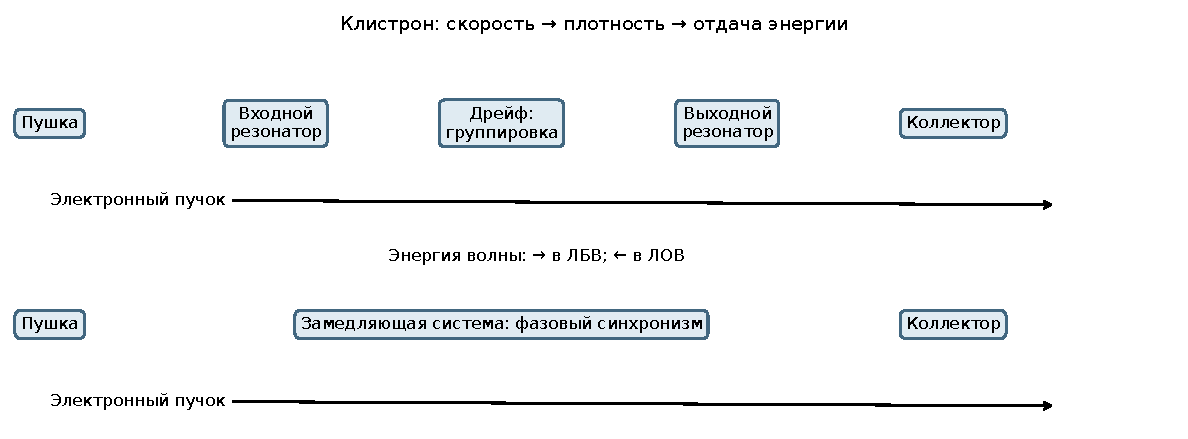
\includegraphics[width=0.92\linewidth]{figures/microwave_devices.pdf}\end{center}

